In this section, I will present experimental results on feature extraction and reason for choosing specific algorithm. I used Intel \emph{OpenCV (Open Source Computer Vision)} library version 2.3 to test the performance of the feature extractors. I developed the algorithms using \emph{C++} in \emph{Microsoft Visual Studio 2010}. I carried out tests in my machine with following configurations:
\begin{itemize}
	\item Operating System: Windows 7 Professional 64 bit
	\item Processor: Intel Core i5 2.80 GHz
	\item Memory: 8.00 GB 	
\end{itemize}

I will focus on the following two measures to select best algorithm:
\begin{description}
\item[Accuracy] The inaccurate stitching result may give false information to the analysts; we choose the algorithm which results best accuracy for medical images. I will check the stability of the detected corners for different intensity, orientation, and scaling.
\item[Computational Complexity] High computational complexity will take longer time to perform a task which is undesirable. We try to get the algorithm which has real time performance. Sometimes, we tweak the algorithms to work faster (parallel processing for example). There is trade-off between computational complexity and accuracy. So, we select the algorithm which is faster and gives acceptable result. 
\end{description}

\noindent I have tested 3 popular feature extractors: Harris, SIFT and SURF. A good corner detector should fulfill certain requirements as discussed in section~\ref{sec:req-corner-detector}, so I will evaluate the feature detectors based upon those requirements i.e. computational time and repeatability rate of key-points for different intensity, orientation, scaled images.\\

\noindent To evaluate the performance of the detectors, I have used the different images mentioned below:
\begin{description}
\item[Normal Image] This is normal X-ray image of resolution 666 x 1024 (i.e. 681984 pixels). This is standard image and I have modified this image to create other different intensity or orientational images. 

\item[High Intensity Image] The pixels of the normal image are increased by 25\% to get high intensity image. The high intensity image and normal image have same number of pixels.
\item[Rotated Image] The normal image rotated by 8\deg and the unassigned pixels have been removed and the image size is 538 x 892 (i.e. 479896 pixels). Thus, the rotated image pixels have been reduced by 30\%.
\item[Scaled Image] The height and width of the normal image are increased to get scaled image. The resulting scaled image size is 1138x1751 (1992638 pixels) which contains nearly double the pixels in the normal image.
\item[Noisy Image] The normal image consists of very little noise. To carry out the tests for noise image, I have added some Gaussian noise (with mean=0, variance=0.001) to the standard image to get the noisy image.
\end{description}

\subsection{Experiment 1: Computational Time}
% Data: Harris: 72.714 54.013 38.076 158.564 53.619
       %SIFT: 402.993 350.434 270.318 1019.413 379.934
			 % SURF: 242.045 240.767 177.066 705.498 244.308                                             
I have estimated the computational time for the feature extractors for different intensity and orientation images mentioned above. The computational time of the key-point detectors has been presented in chart
%measurement(in milliseconds) is presented in table~\ref{table:feature-computational-time} and the chart is 
shown in figure~\ref{fig:feature-computational-time}. \\
%\begin{table}[H]
%\begin{tabular}{l|c|c|c|c|c|}
%\cline{2-6} 
%& \multicolumn{5}{c}{Computing Time(milliseconds)}\\ \cline{2-6}
%& Original & High Intensity  & Rotation & Scale & Noise \\ \hline
%\multicolumn{1}{|c|}{Harris} & 72.714 & 54.013 & 38.076 & 158.564 & 65.919\\ \hline
%\multicolumn{1}{|c|}{SIFT} & 402.993 & 350.434 & 270.318 & 1019.413 & 427.934\\ \hline
%\multicolumn{1}{|c|}{SURF} & 242.045 & 240.767 & 177.066 & 705.498 & 240.308\\ \hline 
%\end{tabular}
%\caption{Computational time of feature detectors}
%\label{table:feature-computational-time}
%\end{table}

\begin{figure}[H]%
\centering
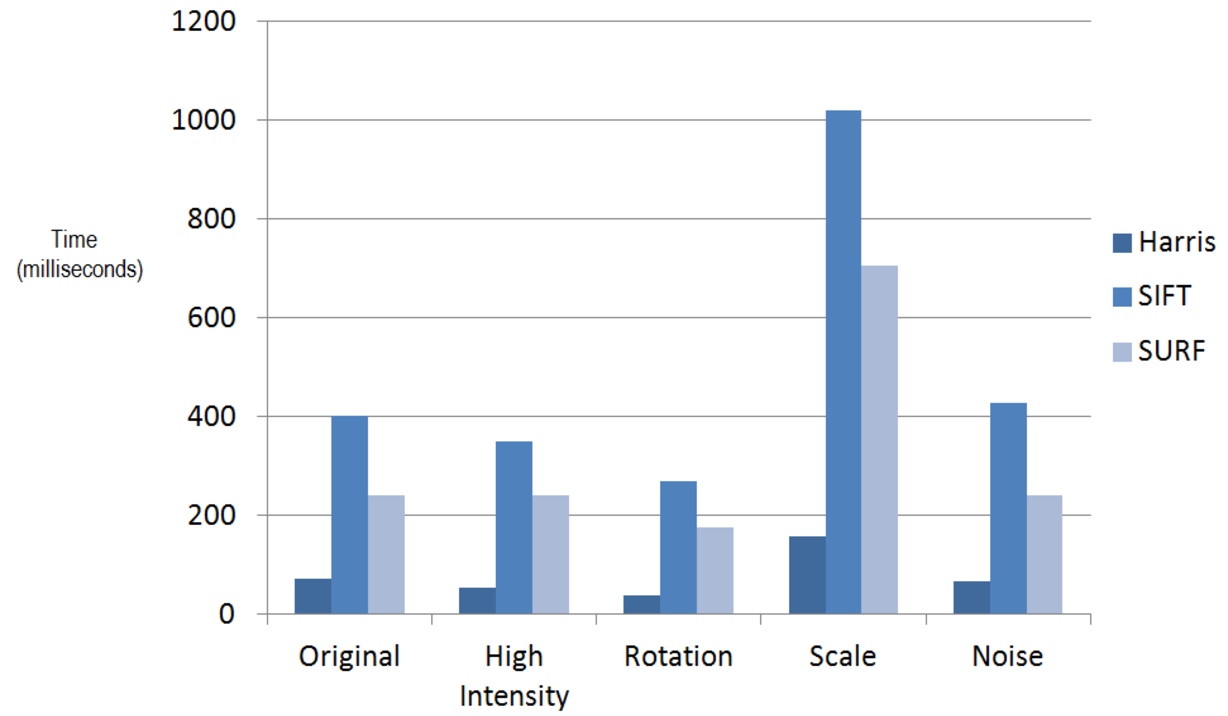
\includegraphics[width=\columnwidth]{2.mainmatter/2.Methodology/FeaturesExtraction/figures/features-CT}%
\caption[Comparison: Computational Time]{Chart showing the computational time (milliseconds) of feature extractors for different images}%
\label{fig:feature-computational-time}%
\end{figure}

\noindent The original, high intensity and noisy images contain same number of pixels; the time taken by the detectors seems similar for those images. For rotated image, the pixels are reduced by 30\%, the computational time also decreases. Similarly, the detectors are slower for scaled image because it contains almost double the number of pixels in original image.\\

\noindent The chart shown in figure~\ref{fig:feature-computational-time} clearly reveals that Harris corner detector is the fastest among detectors and SIFT is the slowest for all types of images. Keeping this in  mind, we go on further experiments to evaluate the accuracy of the feature detectors to figure out the best feature extractor.


\subsection{Experiment 2: Stability}
In this experiment, the stability of the feature detectors is computed for different intensity or orientation images. The stability of the key-point detectors is an important property because it determines the accuracy of the detected key-points. To measure the stability of a key-point detector, we apply key-point detecting algorithm to the standard image (i.e. normal image) and other images; then count the number of key-points. The repeated key-points lie on the same feature location of the standard image. The repeated key-points on the other images are counted. Suppose, we got $N$ key-points in standard image and $N'$ key-points in other image; out of which $N_{repeated}$ are repeated. We estimate the stability of the key-point detector as follows:
\begin{equation}
Stability=\frac{N_{repeated}}{N}
\label{eq:stability}
\end{equation}
The stability is generally expressed in percentage (\%) and the higher the stability the better is the key-point detector. So, we select the feature detector which gives highly stable corners.\\ 

\noindent Table~\ref{table:corners-count} presents the detected key-points count for original image and other variant images. I have included the counts for repeated key-points to estimate the stability of the feature detector.
\begin{table}[H]%
\centering
\begin{tabular}{l|c|c|c|c|c|c|}
\cline{2-7}
&\multicolumn{2}{|c|}{\textbf{HARRIS}} & \multicolumn{2}{|c|}{\textbf{SIFT}} & \multicolumn{2}{|c|}{\textbf{SURF}} \\ \cline{2-7}
& \multicolumn{2}{|c|}{Original image: 245} & \multicolumn{2}{|c|}{Original image: 306} & \multicolumn{2}{|c|}{Original image: 291} \\ \hline
\multicolumn{1}{|c|}{\textbf{Image}} & \textbf{Identified} & \textbf{Repeated} & \textbf{Identified} & \textbf{Repeated} & \textbf{Identified} & \textbf{Repeated} \\ \hline
\multicolumn{1}{|c|}{Brighter} & 183 & 136 & 261 & 225&255 & 234\\ \hline
\multicolumn{1}{|c|}{Rotated} & 173 & 85 & 196 & 139& 177 &125\\ \hline
\multicolumn{1}{|c|}{Scaled} & 481 & 82 &265 & 259& 299 & 164 \\ \hline
\multicolumn{1}{|c|}{Noisy} & 273 & 174 & 488 & 290 & 325 & 214 \\ \hline
\end{tabular}
\caption[Feature Points Count]{Feature points count for stability measurement}
\label{table:corners-count}
\end{table} 

\noindent The count of generated and repeated key-points of the images are used to compute the stability of the feature extractors (using equation~\ref{eq:stability} above). The stability of the key-point detectors for different images has been  presented in chart shown in figure~\ref{fig:repeatability-chart}.

%\begin{table}[H]%
%\centering
%\begin{tabular}{ll|c|c|c|}
%\cline{3-5}
 %&& HARRIS & SIFT & SURF\\ \cline{1-5}
%\multicolumn{1}{|c|} {\multirow{4}{*}{\textbf{Stability(\%)}}} & Brighter & 55.51 & 73.52& 80.41\\ \cline{2-5}
 %  \multicolumn{1}{|c|}{}& Rotated & 34.69 & 45.42& 42.96\\  \cline{2-5}
%		\multicolumn{1}{|c|}{}& Scaled & 33.46 & 84.64 & 56.35 \\ \cline{2-5}
%		\multicolumn{1}{|c|}{}& Noisy & 71.02 & 94.77 & 73.53\\ \hline	
%\end{tabular}
%\caption[Stability measurement]{Stability measurement of the corner detectors}
%\label{table:stability}
%\end{table}


\begin{figure}[H]%
\centering
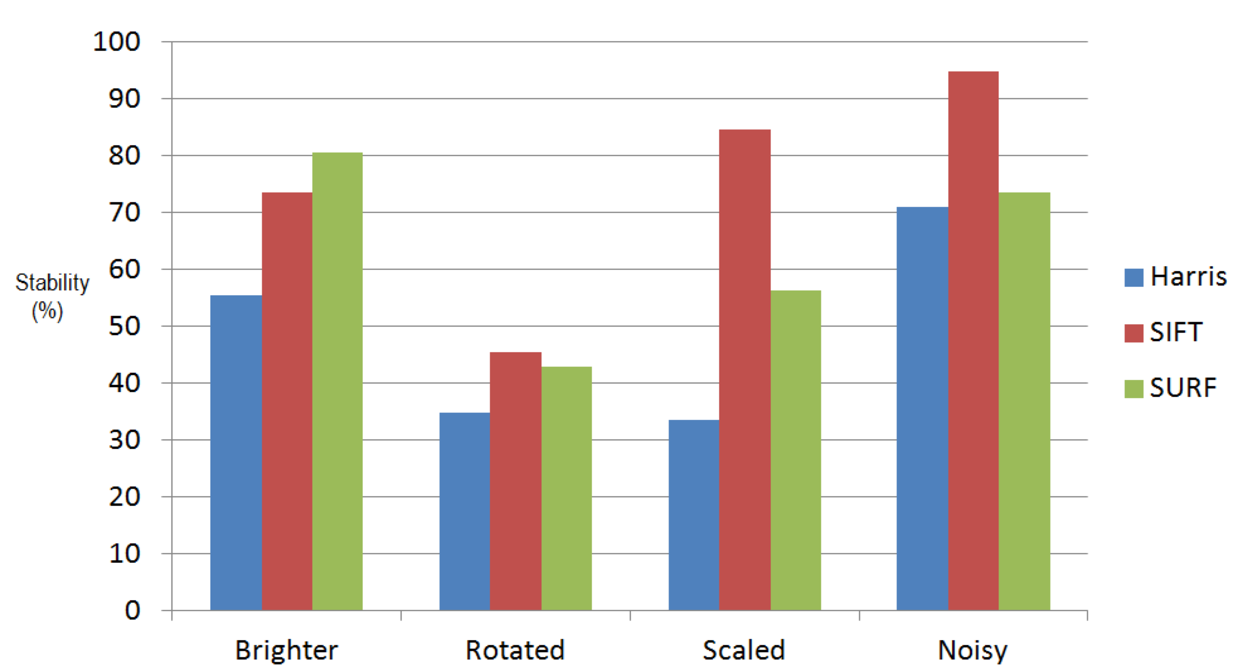
\includegraphics[width=\columnwidth]{2.mainmatter/2.Methodology/FeaturesExtraction/figures/feature-extraction-stability}%
\caption[Comparison: Stability of Corners]{Chart showing the stability of  feature extractors}%
\label{fig:repeatability-chart}%
\end{figure}

\noindent The chart presented in figure~\ref{fig:repeatability-chart} shows that SIFT has high stability for all types of images while Harris giving low stable corners. It is interesting that all key-point detectors have high stability for noisy image. It is because the detectors generate very large number of key-points for noisy image (see table~\ref{table:corners-count}). Therefore, we get higher number of repeated key-points which results higher stability. The less stable key-points for rotated images is because of the decreased size of rotated image i.e. some part of the rotated image is trimmed off to remove unassigned pixels.\\

\noindent In conclusion, Harris corner detector is computationally efficient; but produces less stable key-points which means it generates more inaccurate or inconsistent key-points for different intensity or orientational images. Stability is an important feature for key-point detectors and SIFT and SURF are good to generate highly stable key-points. SIFT is slower but giving highly stable key-points while SURF is faster but less stable than SIFT. So, both SIFT and SURF are chosen as the good key-point detectors. In the next chapter, we will evaluate the matching performance of SIFT and SURF.

%Include the picture of SIFT and SURF with different rotations and scaling. Show the repeatibility with matching points.

% Include the time measure of SIFT and SURF

% Present the comparison chart of Harris, SIFT and SURF
